\documentclass[11pt, a4paper]{article}
\usepackage{polski}
\usepackage[utf8]{inputenc}
\usepackage[T1]{fontenc}
\usepackage[export]{adjustbox}
\usepackage{graphicx}
\usepackage{amsmath} 
\usepackage{listings}
\usepackage{color}
\usepackage{marvosym}
\usepackage{geometry}
\usepackage{float}
\usepackage{booktabs}
\usepackage{multirow}
\usepackage{titlesec}
\usepackage{hyperref}

\geometry{margin=1.2in}
\usepackage[final]{pdfpages}

\newcommand{\fbi}{\leavevmode{\parindent=1em\indent}}

\definecolor{dkgreen}{rgb}{0,0.6,0}
\definecolor{gray}{rgb}{0.5,0.5,0.5}
\definecolor{mauve}{rgb}{0.58,0,0.82}

\lstset{
	frame=tblr,
	language=R,
	aboveskip=3mm,
	belowskip=3mm,
	showstringspaces=false,
	columns=flexible,
	basicstyle={\small\ttfamily},
	numbers=left,
	numberstyle=\tiny\color{gray},
	keywordstyle=\color{blue},
	commentstyle=\color{dkgreen},
	stringstyle=\color{mauve},
	breaklines=true,
	mathescape=false,
	breakatwhitespace=true,
	tabsize=3
}

\renewcommand\lstlistingname{Listing}

\titleclass{\subsubsubsection}{straight}[\subsection]
\newcounter{subsubsubsection}[subsubsection]
\renewcommand\thesubsubsubsection{\thesubsubsection.\arabic{subsubsubsection}}
\renewcommand\theparagraph{\thesubsubsubsection.\arabic{paragraph}}

\titleformat{\subsubsubsection}
  {\normalfont\normalsize\bfseries}{\thesubsubsubsection}{1em}{}
\titlespacing*{\subsubsubsection}
{0pt}{3.25ex plus 1ex minus .2ex}{1.5ex plus .2ex}

\makeatletter
\renewcommand\paragraph{\@startsection{paragraph}{5}{\z@}%
  {3.25ex \@plus1ex \@minus.2ex}%
  {-0em}%
  {\normalfont\normalsize\bfseries}}
\renewcommand\subparagraph{\@startsection{subparagraph}{6}{\parindent}%
  {3.25ex \@plus1ex \@minus .2ex}%
  {-1em}%
  {\normalfont\normalsize\bfseries}}
\def\toclevel@subsubsubsection{4}
\def\toclevel@paragraph{5}
\def\toclevel@paragraph{6}
\def\l@subsubsubsection{\@dottedtocline{4}{7em}{4em}}
\def\l@paragraph{\@dottedtocline{5}{10em}{5em}}
\def\l@subparagraph{\@dottedtocline{6}{14em}{6em}}
\makeatother

\setcounter{secnumdepth}{4}
\setcounter{tocdepth}{4}

\hypersetup{pageanchor=false}

\setlength\parindent{3pt}

\renewcommand{\labelenumi}{\alph{enumi}.} 

\date{\today}

\begin{document}

\begin{titlepage}

\newcommand{\HRule}{\rule{\linewidth}{0.5mm}} 
\center 

\textsc{\LARGE Politechnika Wrocławska}\\[1.5cm] 
\textsc{\Large Inteligencja Obliczeniowa i jej zastosowania}\\[0.5cm] 
\HRule \\[0.5cm]
{ \huge \bfseries Badanie algorytmu genetycznego z zakresu optymalizacji globalnej dla wybranych funkcji testowych}\\[0.5cm] 
\HRule \\[1.6cm]
 
\begin{minipage}{0.4\textwidth}
\begin{flushleft} \large
\emph{Autorzy:}\\
Paweł  \textsc{Andziul} 200648 \\
Marcin  \textsc{Słowiński} 200638 \\
\end{flushleft}
\end{minipage}
~
\begin{minipage}{0.4\textwidth}
\begin{flushright} \large
\emph{Prowadzący:} \\
dr hab. inż. Olgierd \textsc{Unold}, prof. nadzw. PWr
\end{flushright}
\end{minipage}\\[4cm]

\vfill 
{\large 5 kwietnia 2017}\\[3cm] 

\end{titlepage}

\tableofcontents

\newpage
\section{Wprowadzenie}
\paragraph{}
Algorytmy genetyczne to

\fbi
W ramach laboratorium należało przeprowadzić testy algorytmu genetycznego dla różnych parametrów. Jako benchmark oceny należało użyć pakietu ,,getGlobalOpts'' oraz języka R.

\fbi
Pomiary wykonywano na 2 różnych jednostkach roboczych. Ich parametry nie są istotne z punktu widzenia analizy i możliwości porównania rezultatów.

\section{Implementacja}
\paragraph{}
Poniżej (listing ~\ref{lst:skryptGlowny}) zamieszczono kod napisany w języku R przygotowany w celu umożliwienia przeprowadzenia pomiarów.

\lstinputlisting[label=lst:skryptGlowny,caption=Skrypt w języku R wykorzystany do badań,firstline=1,lastline=300]{./assets/skrypt_lab12.R}

\subsection{Parametryzacja skryptu}
Parametryzacji podlega jedynie algorytm genetyczny.
Wybór funkcji do optymalizacji odbywa się przez podanie jej nazwy.
Pozostałe dane są odczytywane z pakietu ,,globalOptTests''.

\section{Przebieg badań}
\paragraph{}
Do badań zostały wybrane funkcje o różnych wymiarach zaczynając na 2 kończąc na 20. Poniżej wymieniono te funkcje wraz z ilością wymiarów podaną w nawiasie.

\begin{itemize}
	\item Branin (2)
	\item Gulf (3)
	\item CosMix4 (4)
	\item EMichalewicz (5)
	\item Hartman6 (6)
	\item PriceTransistor (9)
	\item Schwefel (10)
	\item Zeldasine20 (20)
\end{itemize}

\fbi
Każdy pomiar przeprowadzano 10-krotnie wyniki uśredniając. Domyślne parametry wynosiły kolejno:

\begin{itemize}
	\item rozmiar populacji - 50
	\item liczba iteracji - 100
	\item p. mutacji - 0,1
	\item p. krzyżowania - 0,8
\end{itemize}

\subsection{Branin (2 parametry)}
\paragraph{}
Branin jest funkcją z dwoma parametrami. Na ilustracji (rys.~\ref{fig:branin1}) przedstawiono jej wykres. Wzór funkcji zamieszczono poniżej (\ref{eq:branin}).

\begin{equation}\label{eq:branin}
	f(\boldsymbol{x}) = a(x_2 - bx_1^2 + cx_1 - r)^2 + s(1 - t)\cos(x_1) + s
\end{equation}


\begin{figure}[H]
	\centering
	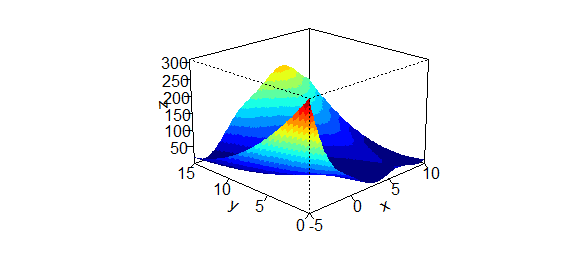
\includegraphics[width=0.9\textwidth]{./assets/branin1.png}
	\caption{Wykres funkcji Branin (d=2)}
	\label{fig:branin1}
\end{figure}

\fbi
Na kolejnych stronach zamieszczono wyniki pomiarów dla różnych wartości parametrów algorytmu genetycznego.

\begin{figure}[H]
	\centering
	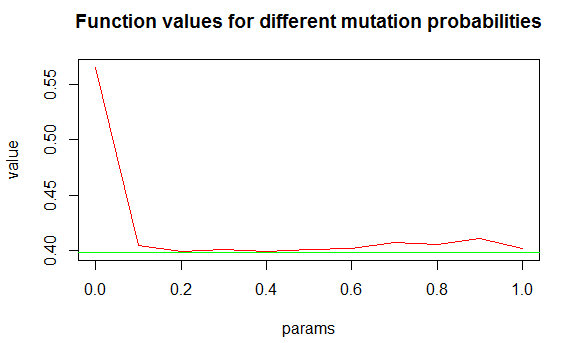
\includegraphics[width=0.9\textwidth]{./assets/branin2.png}
	\caption{Wartość znalezionego optimum w zależności od prawdopodobieństwa mutacji}
	\label{fig:branin2}
\end{figure}

\begin{figure}[H]
	\centering
	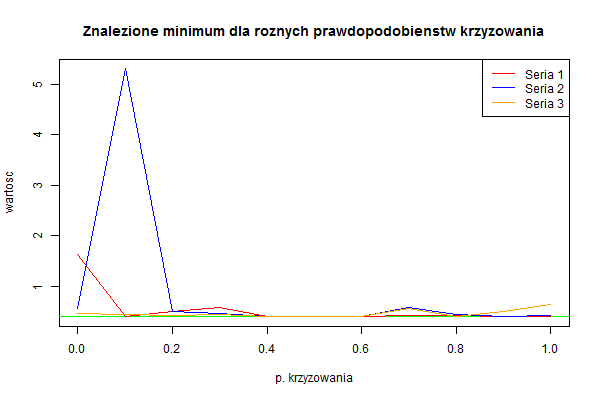
\includegraphics[width=0.9\textwidth]{./assets/branin3.png} % 
	\caption{Wartość znalezionego optimum w zależności od prawdopodobieństwa krzyżowania}
	\label{fig:branin3}
\end{figure}

\begin{figure}[H]
	\centering
	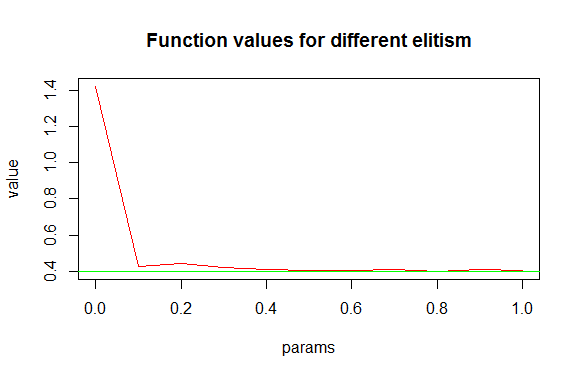
\includegraphics[width=0.9\textwidth]{./assets/branin4.png} % 
	\caption{Wartość znalezionego optimum w zależności od przyjętego elityzmu}
	\label{fig:branin4}
\end{figure}

\begin{figure}[H]
	\centering
	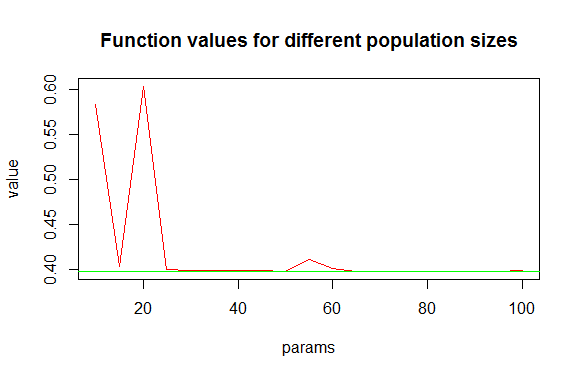
\includegraphics[width=0.9\textwidth]{./assets/branin5.png} % 
	\caption{Wartość znalezionego optimum w zależności od rozmiarów populacji}
	\label{fig:branin5}
\end{figure}

\begin{figure}[H]
	\centering
	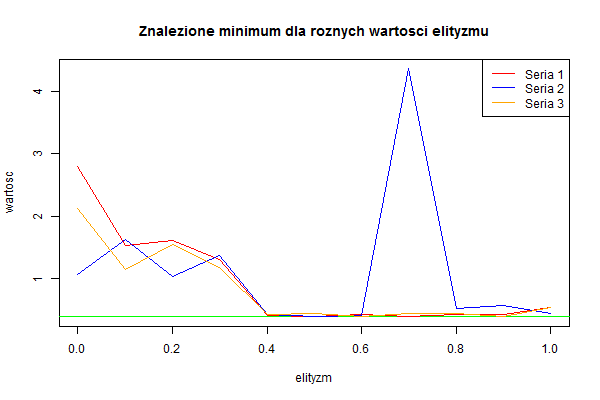
\includegraphics[width=0.9\textwidth]{./assets/branin6.png} % 
	\caption{Wartość znalezionego optimum w zależności od ilości iteracji}
	\label{fig:branin6}
\end{figure}

\begin{figure}[H]
	\centering
	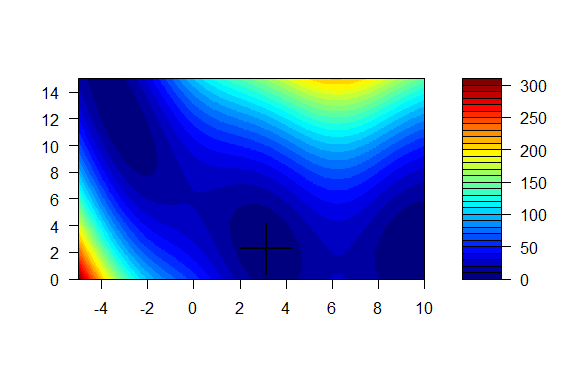
\includegraphics[width=0.9\textwidth]{./assets/branin7.png} % 
	\caption{Poglądowa lokalizacja najlepszego znalezionego optimum}
	\label{fig:branin7}
\end{figure}

\subsection{Gulf (3 parametry)}
\paragraph{}
Gulf jest funkcją przyjmującą trzy parametry. Na ilustracji (rys.~\ref{fig:gulf1}) przedstawiono jej wykres dla pierwszych dwóch wymiarów.

\begin{figure}[H]
	\begin{center}
		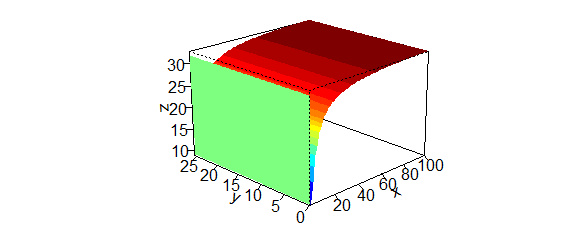
\includegraphics[width=0.9\textwidth]{./assets/gulf1.png} % 
		\caption{Wykres funkcji Gulf (d=3)}
		\label{fig:gulf1}
	\end{center}
\end{figure}

\fbi
Na kolejnych stronach zamieszczono wyniki pomiarów dla różnych wartości parametrów algorytmu genetycznego.

\begin{figure}[H]
	\begin{center}
		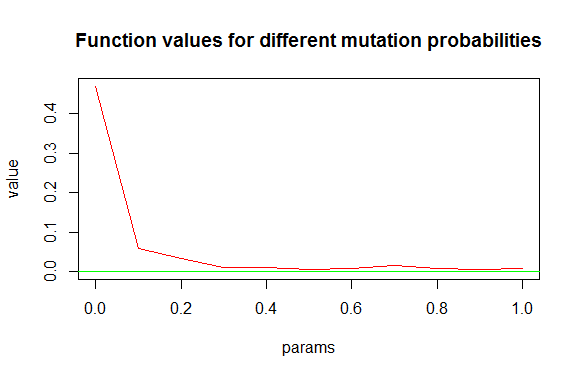
\includegraphics[width=0.9\textwidth]{./assets/gulf2.png} % 
		\caption{Wartość znalezionego optimum w zależności od prawdopodobieństwa mutacji}
		\label{fig:gulf2}
	\end{center}
\end{figure}

\begin{figure}[H]
	\begin{center}
		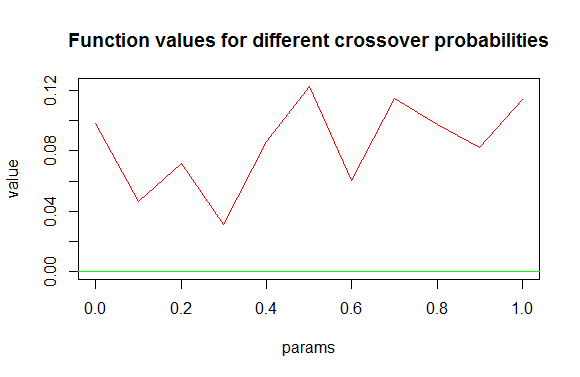
\includegraphics[width=0.9\textwidth]{./assets/gulf3.png} % 
		\caption{Wartość znalezionego optimum w zależności od prawdopodobieństwa krzyżowania}
		\label{fig:gulf3}
	\end{center}
\end{figure}

\begin{figure}[H]
	\begin{center}
		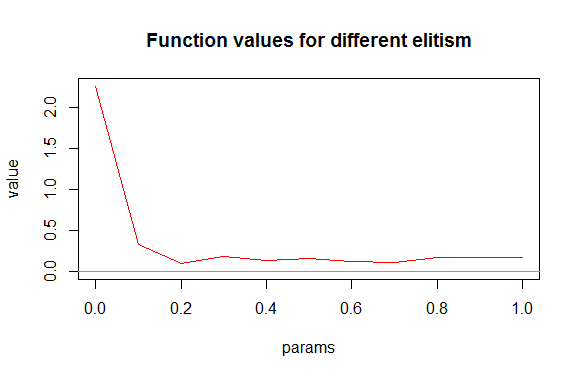
\includegraphics[width=0.9\textwidth]{./assets/gulf4.png} % 
		\caption{Wartość znalezionego optimum w zależności od przyjętego elityzmu}
		\label{fig:gulf4}
	\end{center}
\end{figure}

\begin{figure}[H]
	\begin{center}
		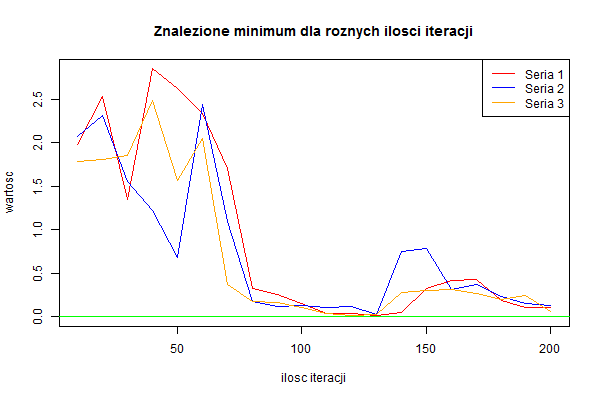
\includegraphics[width=0.9\textwidth]{./assets/gulf5.png} % 
		\caption{Wartość znalezionego optimum w zależności od rozmiarów populacji}
		\label{fig:gulf5}
	\end{center}
\end{figure}

\begin{figure}[H]
	\begin{center}
		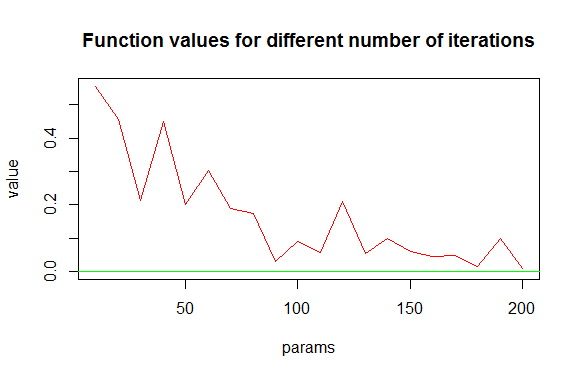
\includegraphics[width=0.9\textwidth]{./assets/gulf6.png} % 
		\caption{Wartość znalezionego optimum w zależności od ilości iteracji}
		\label{fig:gulf6}
	\end{center}
\end{figure}

\fbi
Jak możemy zauważyć na ilustracji poniżej (rys.~\ref{fig:gulf7}) przedstawiona lokalizacja optimum nie jest poprawna, gdyż optymalizacji poddano wersję z 3 parametrami. Ogólnie rzecz biorąc gdyby 3 wymiar przedstawić w postaci gradientu kolorystycznego wtedy byłaby to poprawna lokalizacja niemniej trudna dla intuicyjnego sprawdzenia.

\begin{figure}[H]
	\begin{center}
		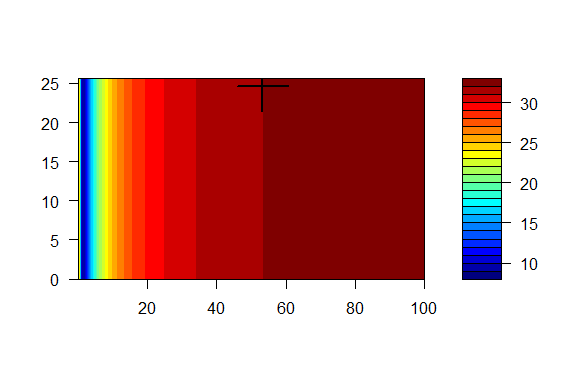
\includegraphics[width=0.9\textwidth]{./assets/gulf7.png} % 
		\caption{Poglądowa lokalizacja najlepszego znalezionego optimum}
		\label{fig:gulf7}
	\end{center}
\end{figure}

\subsection{CosMix4 (4 parametry)}
\paragraph{}


\begin{figure}[H]
	\begin{center}
		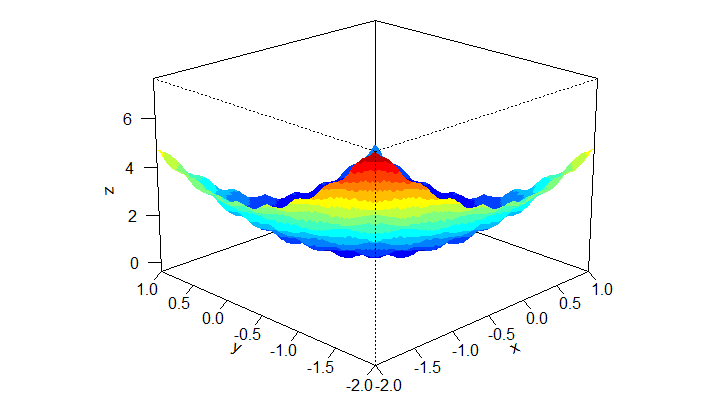
\includegraphics[width=0.9\textwidth]{./assets/CosMix41.png} % 
		\caption{Wykres funkcji CosMix4 (d=4)}
		\label{fig:cosmix41}
	\end{center}
\end{figure}

\begin{figure}[H]
	\begin{center}
		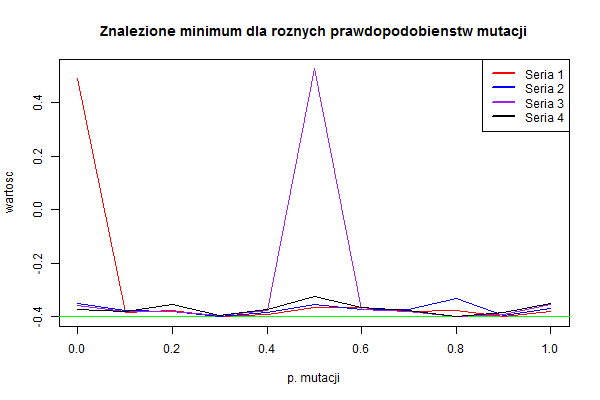
\includegraphics[width=0.9\textwidth]{./assets/CosMix42.png} % 
		\caption{Wartość znalezionego optimum w zależności od prawdopodobieństwa mutacji}
		\label{fig:cosmix42}
	\end{center}
\end{figure}

\begin{figure}[H]
	\begin{center}
		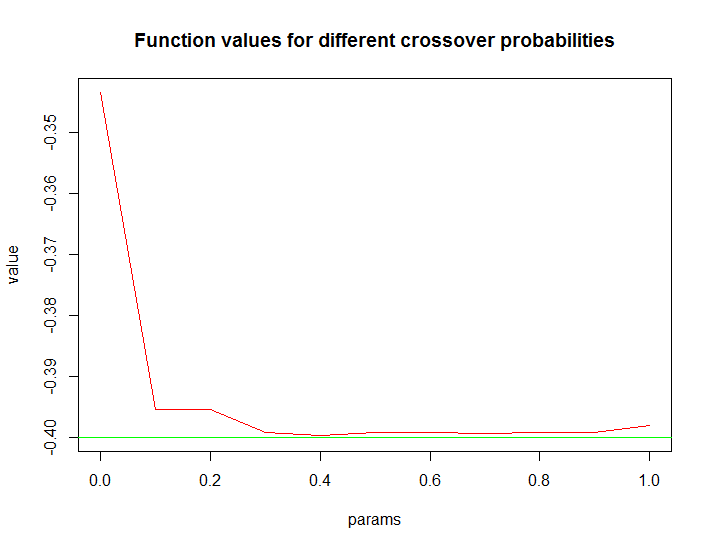
\includegraphics[width=0.9\textwidth]{./assets/CosMix43.png} % 
		\caption{Wartość znalezionego optimum w zależności od prawdopodobieństwa krzyżowania}
		\label{fig:cosmix43}
	\end{center}
\end{figure}

\begin{figure}[H]
	\begin{center}
		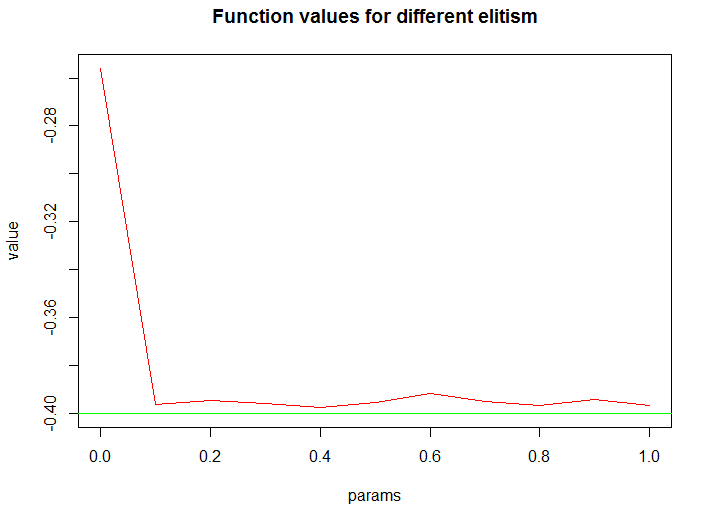
\includegraphics[width=0.9\textwidth]{./assets/CosMix44.png} % 
		\caption{Wartość znalezionego optimum w zależności od przyjętego elityzmu}
		\label{fig:cosmix44}
	\end{center}
\end{figure}

\begin{figure}[H]
	\begin{center}
		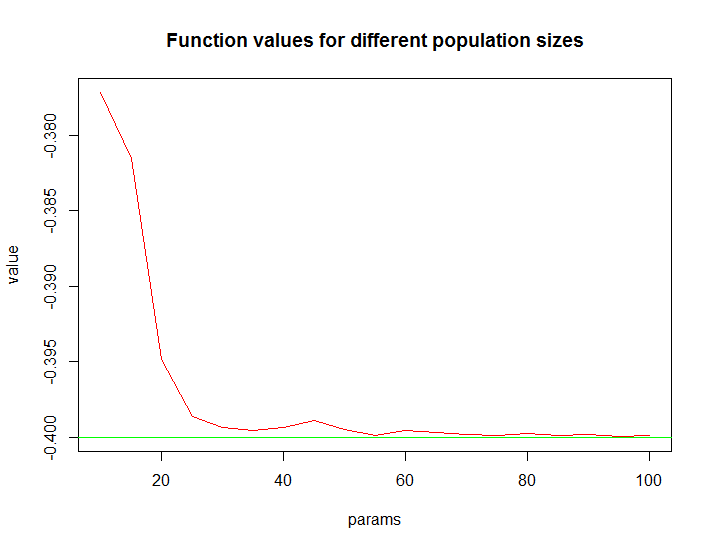
\includegraphics[width=0.9\textwidth]{./assets/CosMix45.png} % 
		\caption{Wartość znalezionego optimum w zależności od rozmiarów populacji}
		\label{fig:cosmix45}
	\end{center}
\end{figure}

\begin{figure}[H]
	\begin{center}
		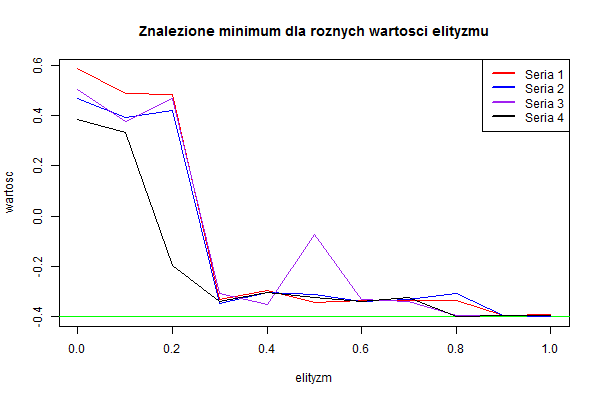
\includegraphics[width=0.9\textwidth]{./assets/CosMix46.png} % 
		\caption{Wartość znalezionego optimum w zależności od ilości iteracji}
		\label{fig:cosmix46}
	\end{center}
\end{figure}

\begin{figure}[H]
	\begin{center}
		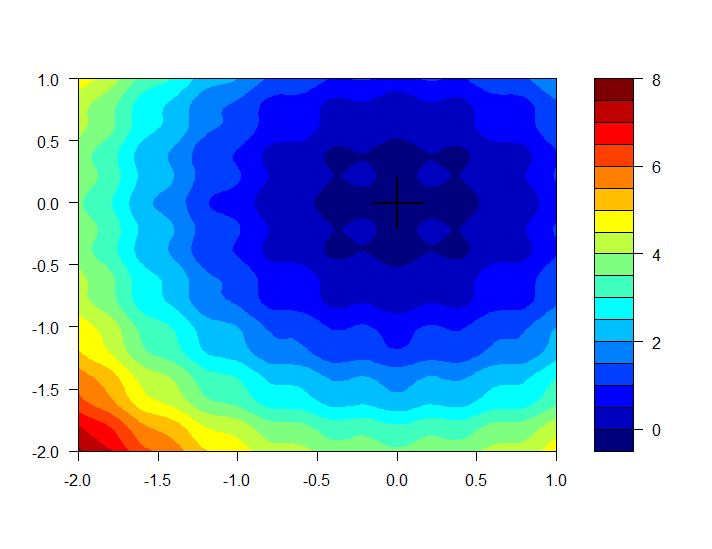
\includegraphics[width=0.9\textwidth]{./assets/CosMix47.png} % 
		\caption{Poglądowa lokalizacja najlepszego znalezionego optimum}
		\label{fig:cosmix47}
	\end{center}
\end{figure}

\subsection{EMichalewicz (5 parametrów)}
\paragraph{}


\begin{figure}[H]
	\begin{center}
		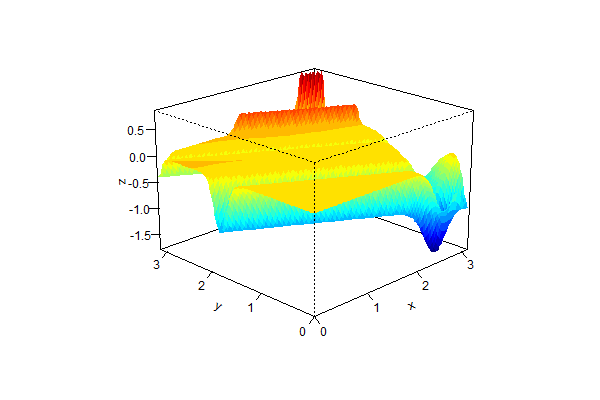
\includegraphics[width=0.9\textwidth]{./assets/EMichalewicz1.png} % 
		\caption{Wykres funkcji EMIchalewicz (d=5)}
		\label{fig:emichalewicz1}
	\end{center}
\end{figure}

\begin{figure}[H]
	\begin{center}
		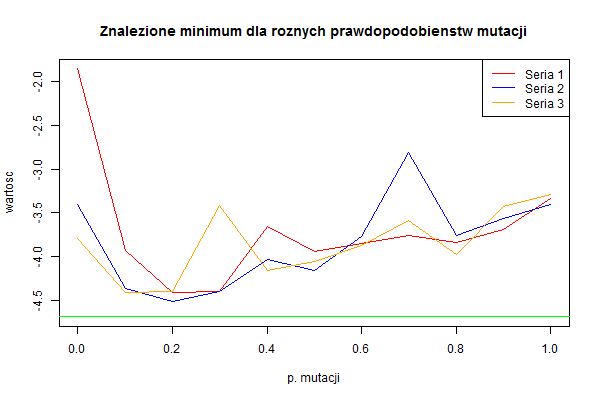
\includegraphics[width=0.9\textwidth]{./assets/EMichalewicz2.png} % 
		\caption{Wartość znalezionego optimum w zależności od prawdopodobieństwa mutacji}
		\label{fig:emichalewicz2}
	\end{center}
\end{figure}

\begin{figure}[H]
	\begin{center}
		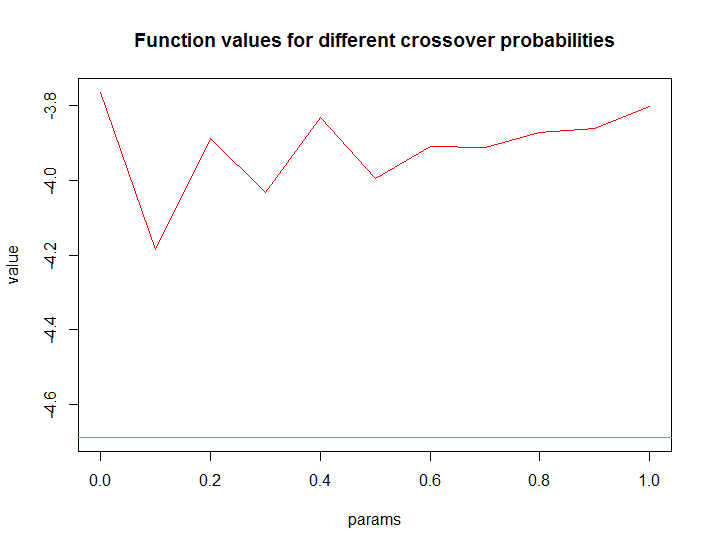
\includegraphics[width=0.9\textwidth]{./assets/EMichalewicz3.png} % 
		\caption{Wartość znalezionego optimum w zależności od prawdopodobieństwa krzyżowania}
		\label{fig:emichalewicz3}
	\end{center}
\end{figure}

\begin{figure}[H]
	\begin{center}
		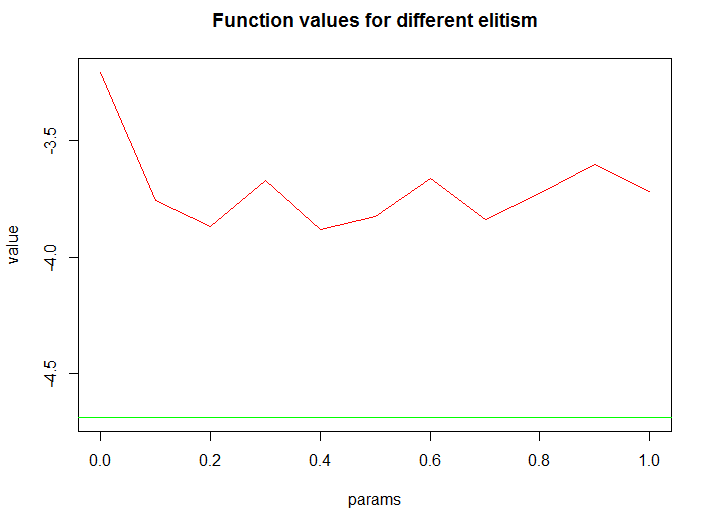
\includegraphics[width=0.9\textwidth]{./assets/EMichalewicz4.png} % 
		\caption{Wartość znalezionego optimum w zależności od przyjętego elityzmu}
		\label{fig:emichalewicz4}
	\end{center}
\end{figure}

\begin{figure}[H]
	\begin{center}
		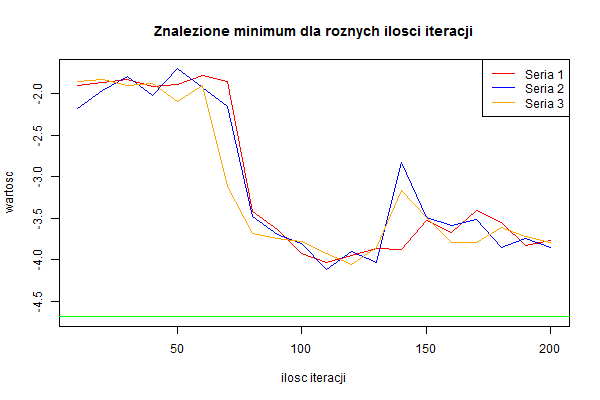
\includegraphics[width=0.9\textwidth]{./assets/EMichalewicz5.png} % 
		\caption{Wartość znalezionego optimum w zależności od rozmiarów populacji}
		\label{fig:emichalewicz5}
	\end{center}
\end{figure}

\begin{figure}[H]
	\begin{center}
		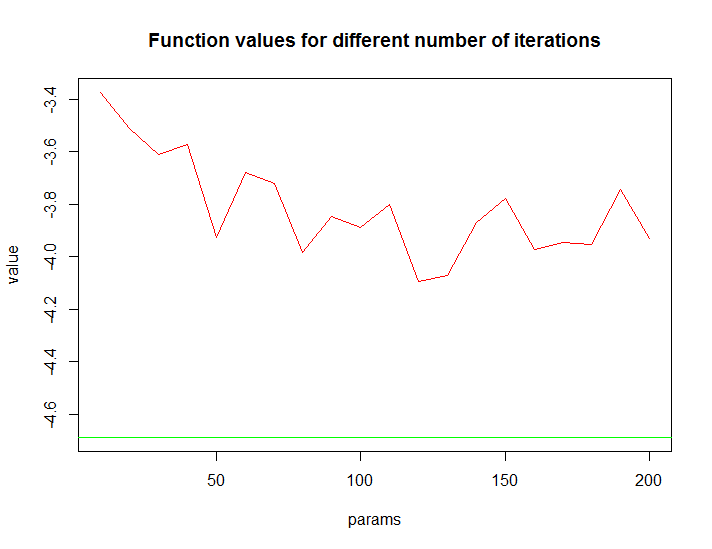
\includegraphics[width=0.9\textwidth]{./assets/EMichalewicz6.png} % 
		\caption{Wartość znalezionego optimum w zależności od ilości iteracji}
		\label{fig:emichalewicz6}
	\end{center}
\end{figure}

\begin{figure}[H]
	\begin{center}
		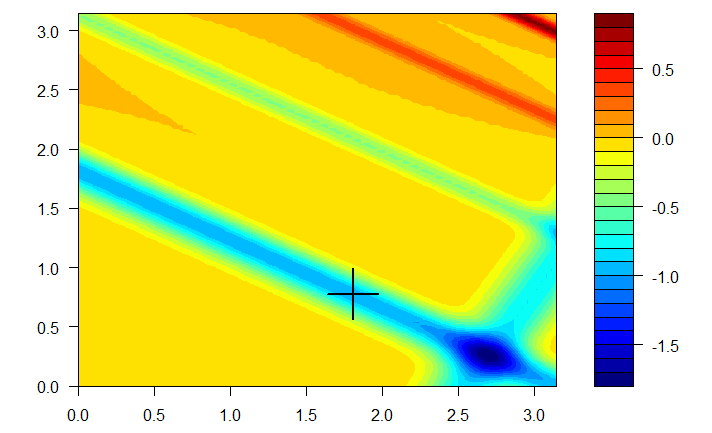
\includegraphics[width=0.9\textwidth]{./assets/EMichalewicz7.png} % 
		\caption{Poglądowa lokalizacja najlepszego znalezionego optimum}
		\label{fig:emichalewicz7}
	\end{center}
\end{figure}

\subsection{Hartman6 (6 parametrów)}
\paragraph{}


\begin{figure}[H]
	\begin{center}
		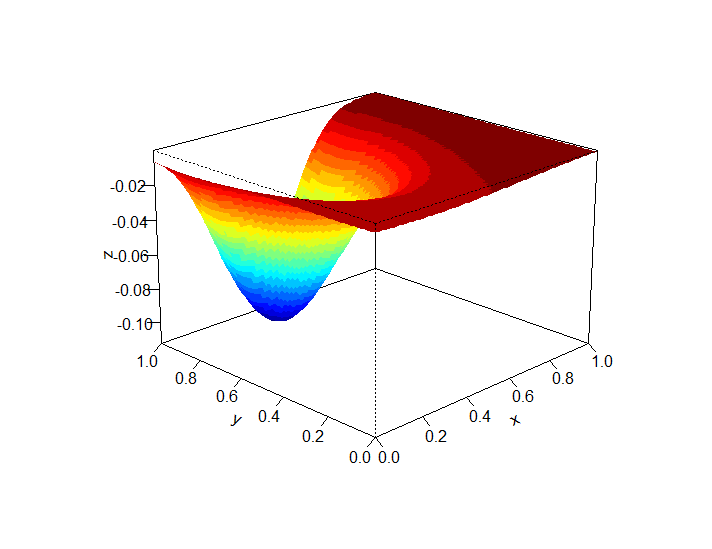
\includegraphics[width=0.9\textwidth]{./assets/Hartman61.png} % 
		\caption{Wykres funkcji Hartman6 (d=6)}
		\label{fig:hartman61}
	\end{center}
\end{figure}

\begin{figure}[H]
	\begin{center}
		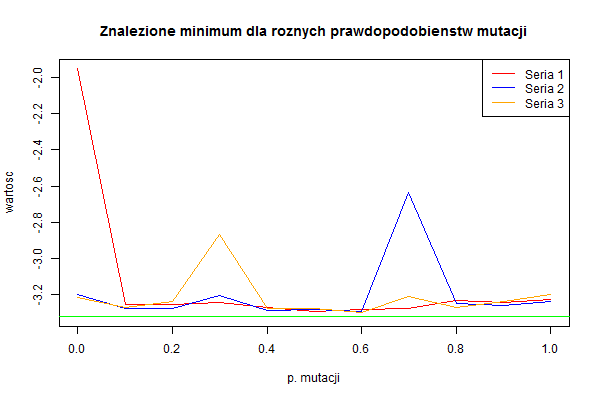
\includegraphics[width=0.9\textwidth]{./assets/Hartman62.png} % 
		\caption{Wartość znalezionego optimum w zależności od prawdopodobieństwa mutacji}
		\label{fig:hartman62}
	\end{center}
\end{figure}

\begin{figure}[H]
	\begin{center}
		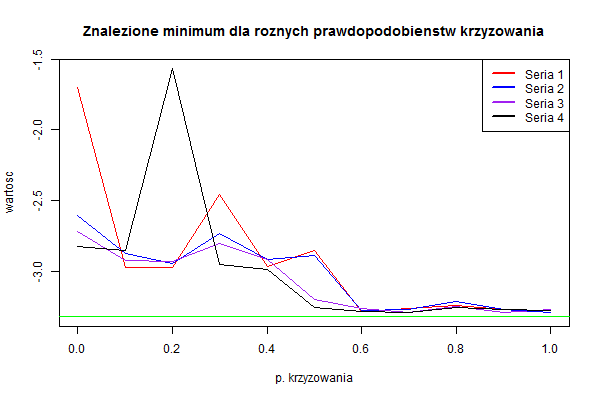
\includegraphics[width=0.9\textwidth]{./assets/Hartman63.png} % 
		\caption{Wartość znalezionego optimum w zależności od prawdopodobieństwa krzyżowania}
		\label{fig:hartman63}
	\end{center}
\end{figure}

\begin{figure}[H]
	\begin{center}
		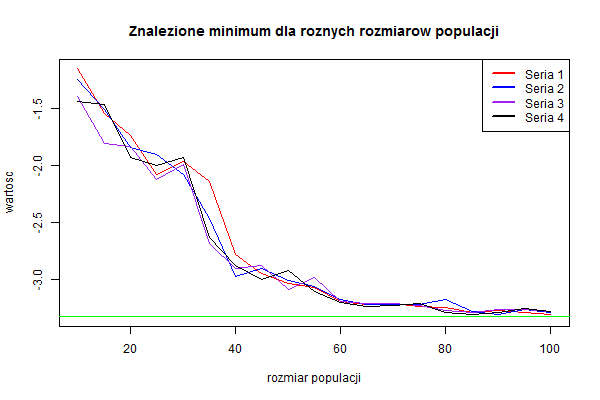
\includegraphics[width=0.9\textwidth]{./assets/Hartman64.png} % 
		\caption{Wartość znalezionego optimum w zależności od przyjętego elityzmu}
		\label{fig:hartman64}
	\end{center}
\end{figure}

\begin{figure}[H]
	\begin{center}
		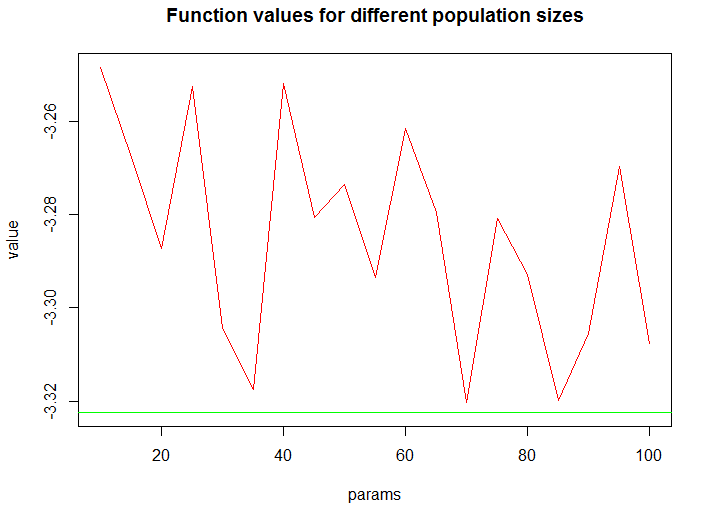
\includegraphics[width=0.9\textwidth]{./assets/Hartman65.png} % 
		\caption{Wartość znalezionego optimum w zależności od rozmiarów populacji}
		\label{fig:hartman65}
	\end{center}
\end{figure}

\begin{figure}[H]
	\begin{center}
		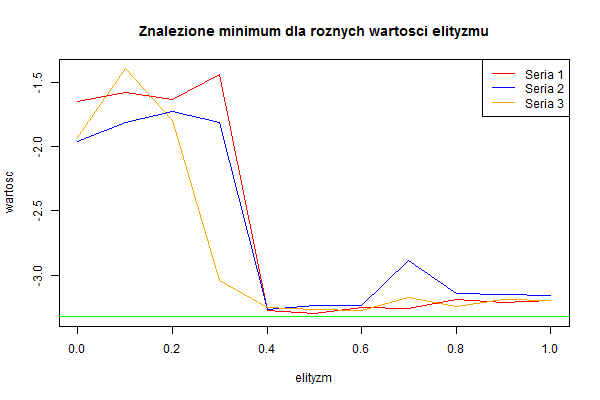
\includegraphics[width=0.9\textwidth]{./assets/Hartman66.png} % 
		\caption{Wartość znalezionego optimum w zależności od ilości iteracji}
		\label{fig:hartman66}
	\end{center}
\end{figure}

\begin{figure}[H]
	\begin{center}
		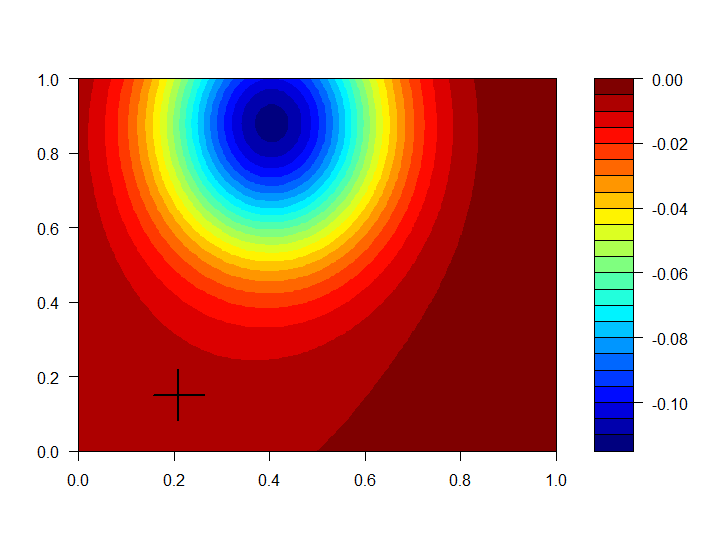
\includegraphics[width=0.9\textwidth]{./assets/Hartman67.png} % 
		\caption{Poglądowa lokalizacja najlepszego znalezionego optimum}
		\label{fig:hartman67}
	\end{center}
\end{figure}

\subsection{PriceTransistor (9 parametrów)}
\paragraph{}


\begin{figure}[H]
	\begin{center}
		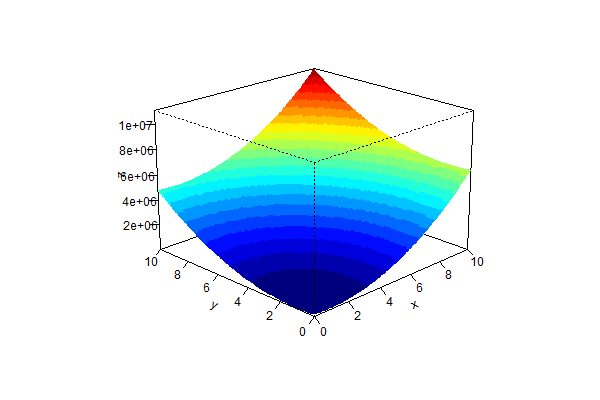
\includegraphics[width=0.9\textwidth]{./assets/PriceTransistor1.png} % 
		\caption{Wykres funkcji PriceTransistor (d=9)}
		\label{fig:pricetransistor1}
	\end{center}
\end{figure}

\begin{figure}[H]
	\begin{center}
		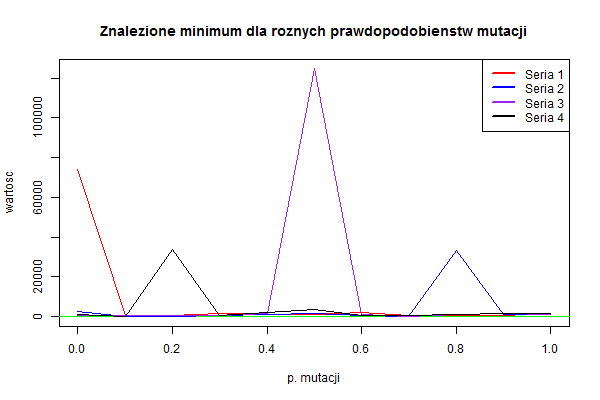
\includegraphics[width=0.9\textwidth]{./assets/PriceTransistor2.png} % 
		\caption{Wartość znalezionego optimum w zależności od prawdopodobieństwa mutacji}
		\label{fig:pricetransistor2}
	\end{center}
\end{figure}

\begin{figure}[H]
	\begin{center}
		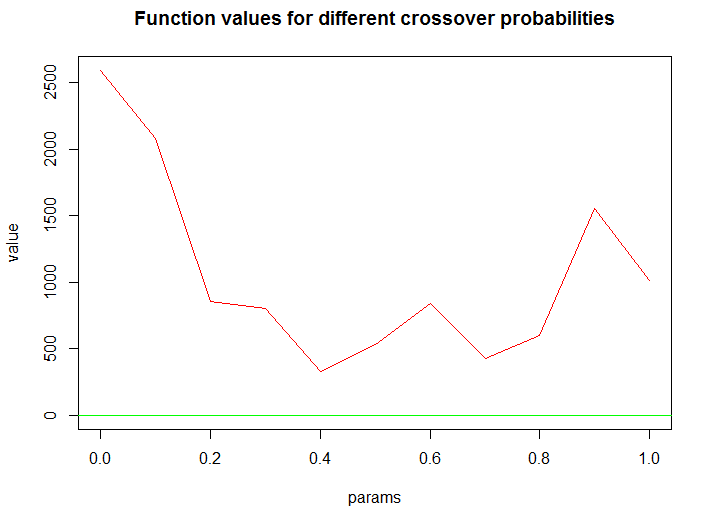
\includegraphics[width=0.9\textwidth]{./assets/PriceTransistor3.png} % 
		\caption{Wartość znalezionego optimum w zależności od prawdopodobieństwa krzyżowania}
		\label{fig:pricetransistor3}
	\end{center}
\end{figure}

\begin{figure}[H]
	\begin{center}
		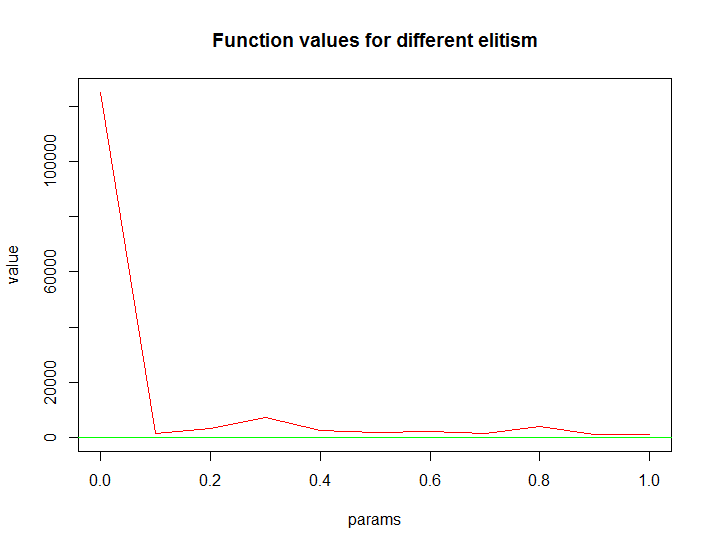
\includegraphics[width=0.9\textwidth]{./assets/PriceTransistor4.png} % 
		\caption{Wartość znalezionego optimum w zależności od przyjętego elityzmu}
		\label{fig:pricetransistor4}
	\end{center}
\end{figure}

\begin{figure}[H]
	\begin{center}
		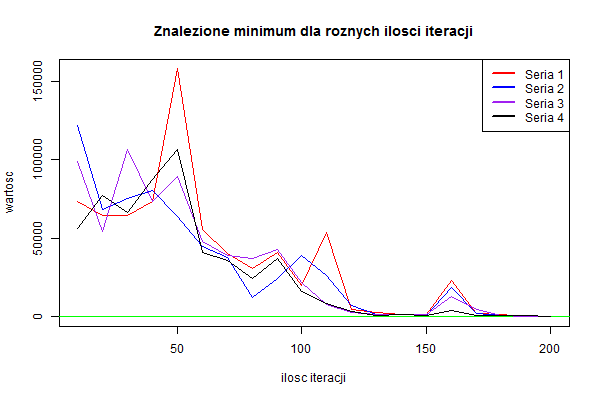
\includegraphics[width=0.9\textwidth]{./assets/PriceTransistor5.png} % 
		\caption{Wartość znalezionego optimum w zależności od rozmiarów populacji}
		\label{fig:pricetransistor5}
	\end{center}
\end{figure}

\begin{figure}[H]
	\begin{center}
		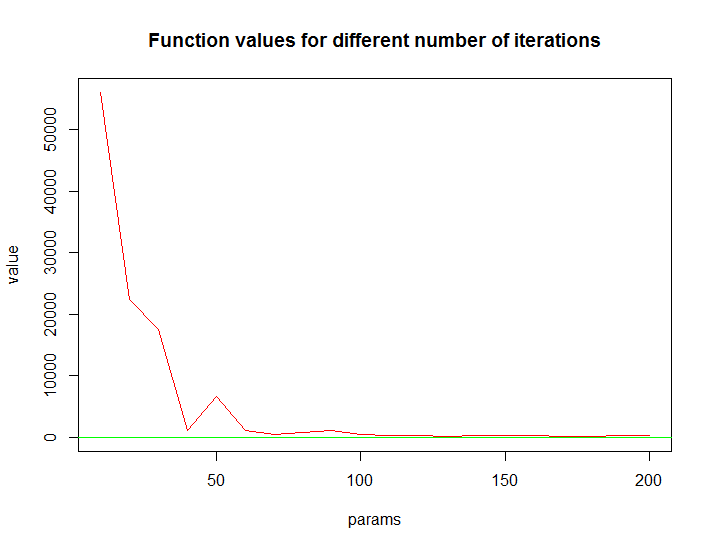
\includegraphics[width=0.9\textwidth]{./assets/PriceTransistor6.png} % 
		\caption{Wartość znalezionego optimum w zależności od ilości iteracji}
		\label{fig:pricetransistor6}
	\end{center}
\end{figure}

\begin{figure}[H]
	\begin{center}
		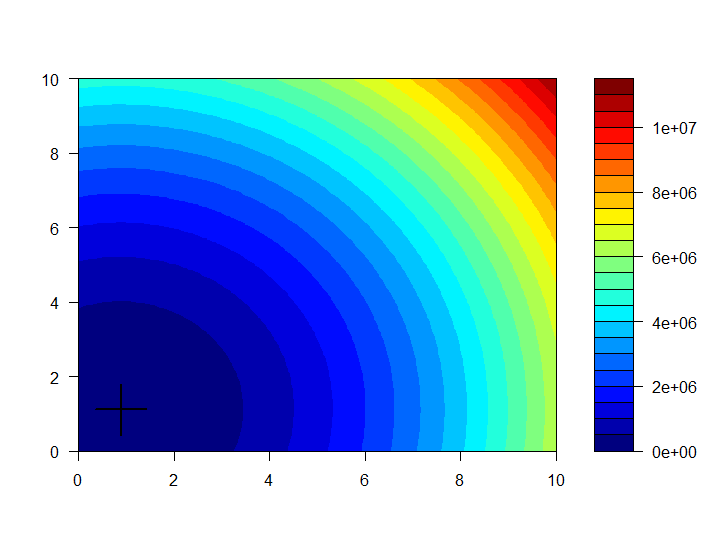
\includegraphics[width=0.9\textwidth]{./assets/PriceTransistor7.png} % 
		\caption{Poglądowa lokalizacja najlepszego znalezionego optimum}
		\label{fig:pricetransistor7}
	\end{center}
\end{figure}

\subsection{Schwefel (10 parametrów)}
\paragraph{}


\begin{figure}[H]
	\begin{center}
		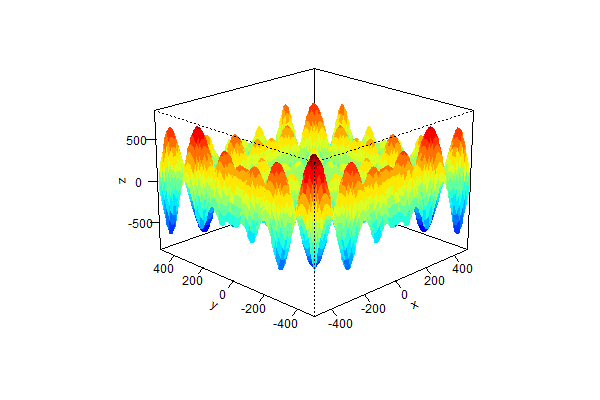
\includegraphics[width=0.9\textwidth]{./assets/Schwefel1.png} % 
		\caption{Wykres funkcji Schwefel (d=10)}
		\label{fig:schwefel1}
	\end{center}
\end{figure}

\begin{figure}[H]
	\begin{center}
		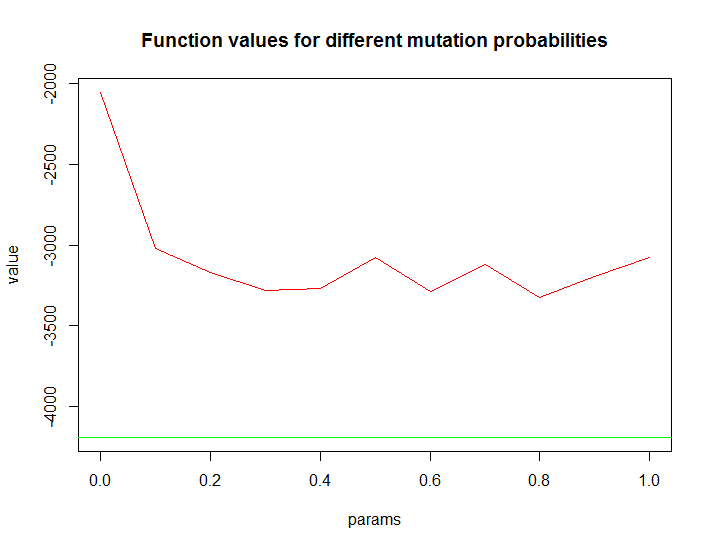
\includegraphics[width=0.9\textwidth]{./assets/Schwefel2.png} % 
		\caption{Wartość znalezionego optimum w zależności od prawdopodobieństwa mutacji}
		\label{fig:schwefel2}
	\end{center}
\end{figure}

\begin{figure}[H]
	\begin{center}
		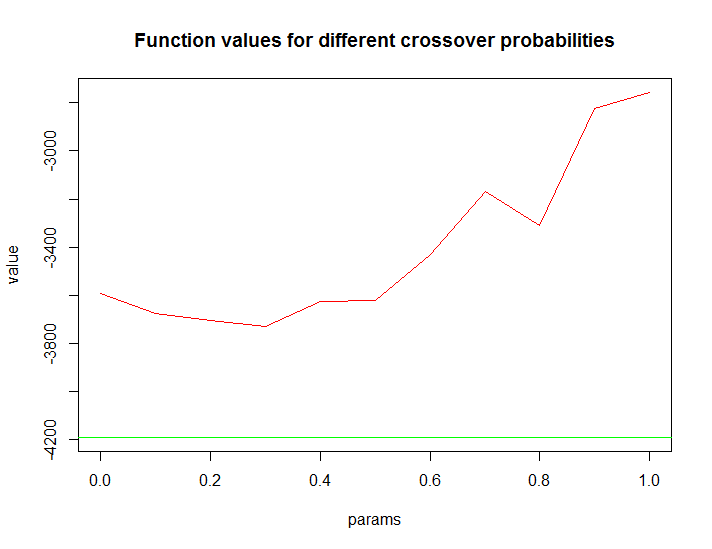
\includegraphics[width=0.9\textwidth]{./assets/Schwefel3.png} % 
		\caption{Wartość znalezionego optimum w zależności od prawdopodobieństwa krzyżowania}
		\label{fig:schwefel3}
	\end{center}
\end{figure}

\begin{figure}[H]
	\begin{center}
		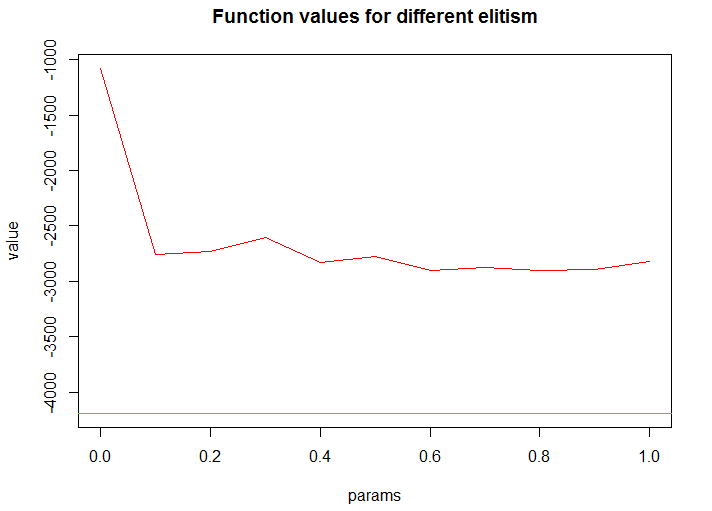
\includegraphics[width=0.9\textwidth]{./assets/Schwefel4.png} % 
		\caption{Wartość znalezionego optimum w zależności od przyjętego elityzmu}
		\label{fig:schwefel4}
	\end{center}
\end{figure}

\begin{figure}[H]
	\begin{center}
		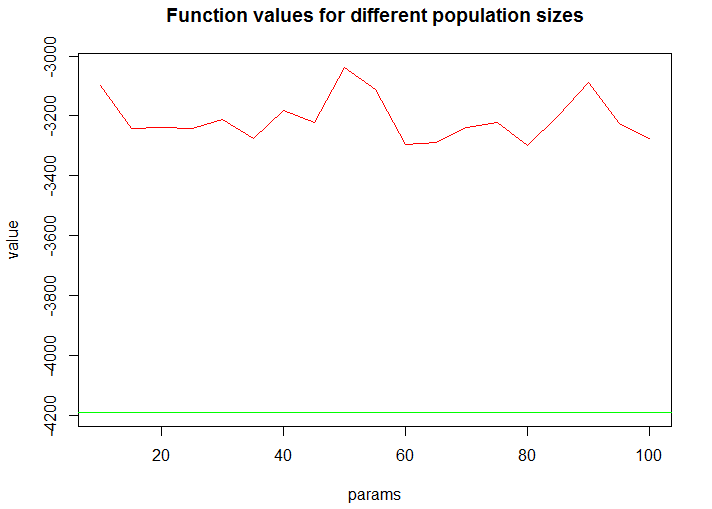
\includegraphics[width=0.9\textwidth]{./assets/Schwefel5.png} % 
		\caption{Wartość znalezionego optimum w zależności od rozmiarów populacji}
		\label{fig:schwefel5}
	\end{center}
\end{figure}

\begin{figure}[H]
	\begin{center}
		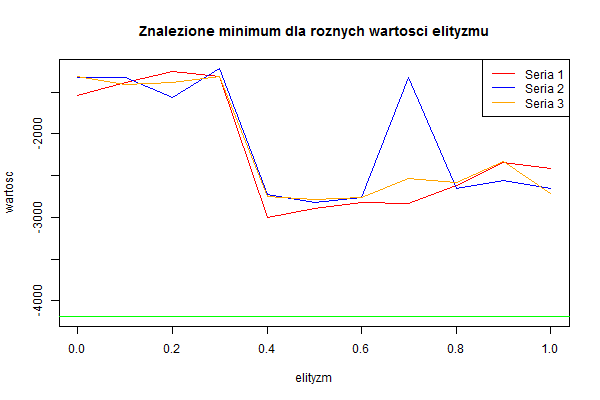
\includegraphics[width=0.9\textwidth]{./assets/Schwefel6.png} % 
		\caption{Wartość znalezionego optimum w zależności od ilości iteracji}
		\label{fig:schwefel6}
	\end{center}
\end{figure}

\begin{figure}[H]
	\begin{center}
		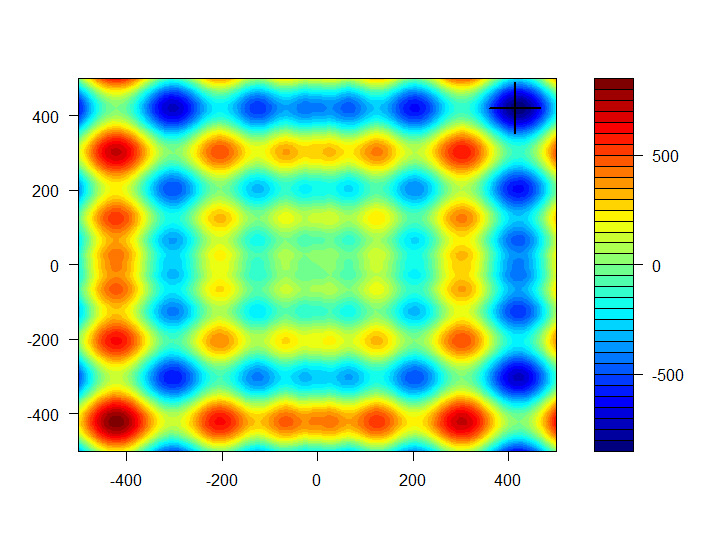
\includegraphics[width=0.9\textwidth]{./assets/Schwefel7.png} % 
		\caption{Poglądowa lokalizacja najlepszego znalezionego optimum}
		\label{fig:schwefel7}
	\end{center}
\end{figure}

\subsection{Zeldasine20 (20 parametrów)}
\paragraph{}


\begin{figure}[H]
	\begin{center}
		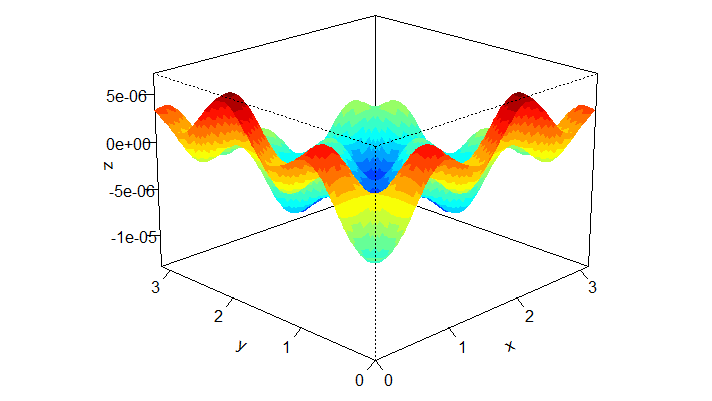
\includegraphics[width=0.9\textwidth]{./assets/Zeldasine1.png} % 
		\caption{Wykres funkcji Zeldasine (d=20)}
		\label{fig:zeldasine1}
	\end{center}
\end{figure}

\begin{figure}[H]
	\begin{center}
		\includegraphics[width=0.9\textwidth]{./assets/Zeldasine2.png} % 
		\caption{Wartość znalezionego optimum w zależności od prawdopodobieństwa mutacji}
		\label{fig:zeldasine2}
	\end{center}
\end{figure}

\begin{figure}[H]
	\begin{center}
		\includegraphics[width=0.9\textwidth]{./assets/Zeldasine3.png} % 
		\caption{Wartość znalezionego optimum w zależności od prawdopodobieństwa krzyżowania}
		\label{fig:zeldasine3}
	\end{center}
\end{figure}

\begin{figure}[H]
	\begin{center}
		\includegraphics[width=0.9\textwidth]{./assets/Zeldasine4.png} % 
		\caption{Wartość znalezionego optimum w zależności od przyjętego elityzmu}
		\label{fig:zeldasine4}
	\end{center}
\end{figure}

\begin{figure}[H]
	\begin{center}
		\includegraphics[width=0.9\textwidth]{./assets/Zeldasine5.png} % 
		\caption{Wartość znalezionego optimum w zależności od rozmiarów populacji}
		\label{fig:zeldasine5}
	\end{center}
\end{figure}

\begin{figure}[H]
	\begin{center}
		\includegraphics[width=0.9\textwidth]{./assets/Zeldasine6.png} % 
		\caption{Wartość znalezionego optimum w zależności od ilości iteracji}
		\label{fig:zeldasine6}
	\end{center}
\end{figure}

\begin{figure}[H]
	\begin{center}
		\includegraphics[width=0.9\textwidth]{./assets/Zeldasine7.png} % 
		\caption{Poglądowa lokalizacja najlepszego znalezionego optimum}
		\label{fig:zeldasine7}
	\end{center}
\end{figure}

\section{Podsumowanie}
\paragraph{}
Test

\fbi
Akapit



\newpage
\begin{thebibliography}{40}

\bibitem{test1}
Artur Suchwałko “Wprowadzenie do R dla programistów innych języków” https://cran.r-project.org/doc/contrib/R-dla-programistow-innych-jezykow.pdf

\end{thebibliography}

\end{document}